\documentclass{beamer}

\mode<presentation>

\title{Symbolic Music Similarity}
\subtitle{Presentation}
\author{Ali Bektas \and Paul Kröger}

\usepackage{graphicx}
\graphicspath{{./images/}}

\usepackage{verbatim}
\setbeameroption{show notes}
%\usepackage{media9}
%\addmediapath{./audio_files/}

\usepackage{mathtools}

\usetheme{Antibes}
\setbeamertemplate{section in toc}[sections numbered]
\setbeamertemplate{subsection in toc}[subsections numbered]


\AtBeginSubsection[]
{
   \begin{frame}
        \frametitle{Inhalts\"ubersicht}
        \tableofcontents[currentsection,currentsubsection]
   \end{frame}
}

\begin{document}
	
	\begin{frame}\maketitle \end{frame}
	\begin{frame}{Überblick} \tableofcontents \end{frame}

	\section{Grundlegendes}

	\begin{frame}
  		\frametitle{Darstellung von Noten}
  		\begin{minipage}{0.45\textwidth}
  			\begin{itemize}
			\item Melodie : \textit{"singbare, in sich geschlossene Folge von Tönen"} \cite{duden_melodie}
			\item Harmonie : \textit{"wohltönender Zusammenklang mehrerer Töne oder Akkorde"} \cite{duden_harmonie}
			\item Schlüssel : \textit{"dient in der Musiknotation dazu, im Notensystem festzulegen, welche Tonhöhe die fünf Notenlinien repräsentieren."} \cite{def_schlussel}
			\note[item]<1>{Das bedeutet für uns immer ein Ton zu einer bestimmten Zeit.}
			\note[item]<1>{In sich geschlossene Folge von Tönen hängt mit Harmonie zusammen.}
			\end{itemize}
		\end{minipage}%
		\begin{minipage}{0.45\textwidth}
			\begin{figure}[h!]
				\includegraphics[width=100px,height=100px,keepaspectratio]{clefs_chord.png}
				\caption{Source: \cite{def_schlussel}}
			\end{figure}
		\end{minipage}
	\end{frame}

	\begin{frame}
		\frametitle{Darstellung von Noten}
			\textit{"Representing music as a weighted point set in a two-dimensional space has a tradition of many centuries. Since approximately the 10th century, one popular way of writing music has been to use a set of notes (points) in a two-dimensional space, with time and pitch as coordinates."}\cite{three}

		\note[item]<1>{In diesem Kontext kann "Gewicht" vieles sein: Die Position einer Note im Takt , die Länge einer Note im Takt , usw.}
		
	\end{frame}



	\begin{frame}
		\frametitle{Darstellung von Noten}
		\begin{itemize}
			\item Rhytmus
			\item Tonlage 
			\item und vieles mehr
			\end{itemize}
	
			\note[item]<1>{Notendarstellung heißt nicht nur , zu welcher Zeit ein Ton gespielt wird , sondern auch , Informationen über , Gefühl beim Spielen , vortragsbetreffliche Elemente zu übermitteln.}
		
		\begin{figure}[h!]
			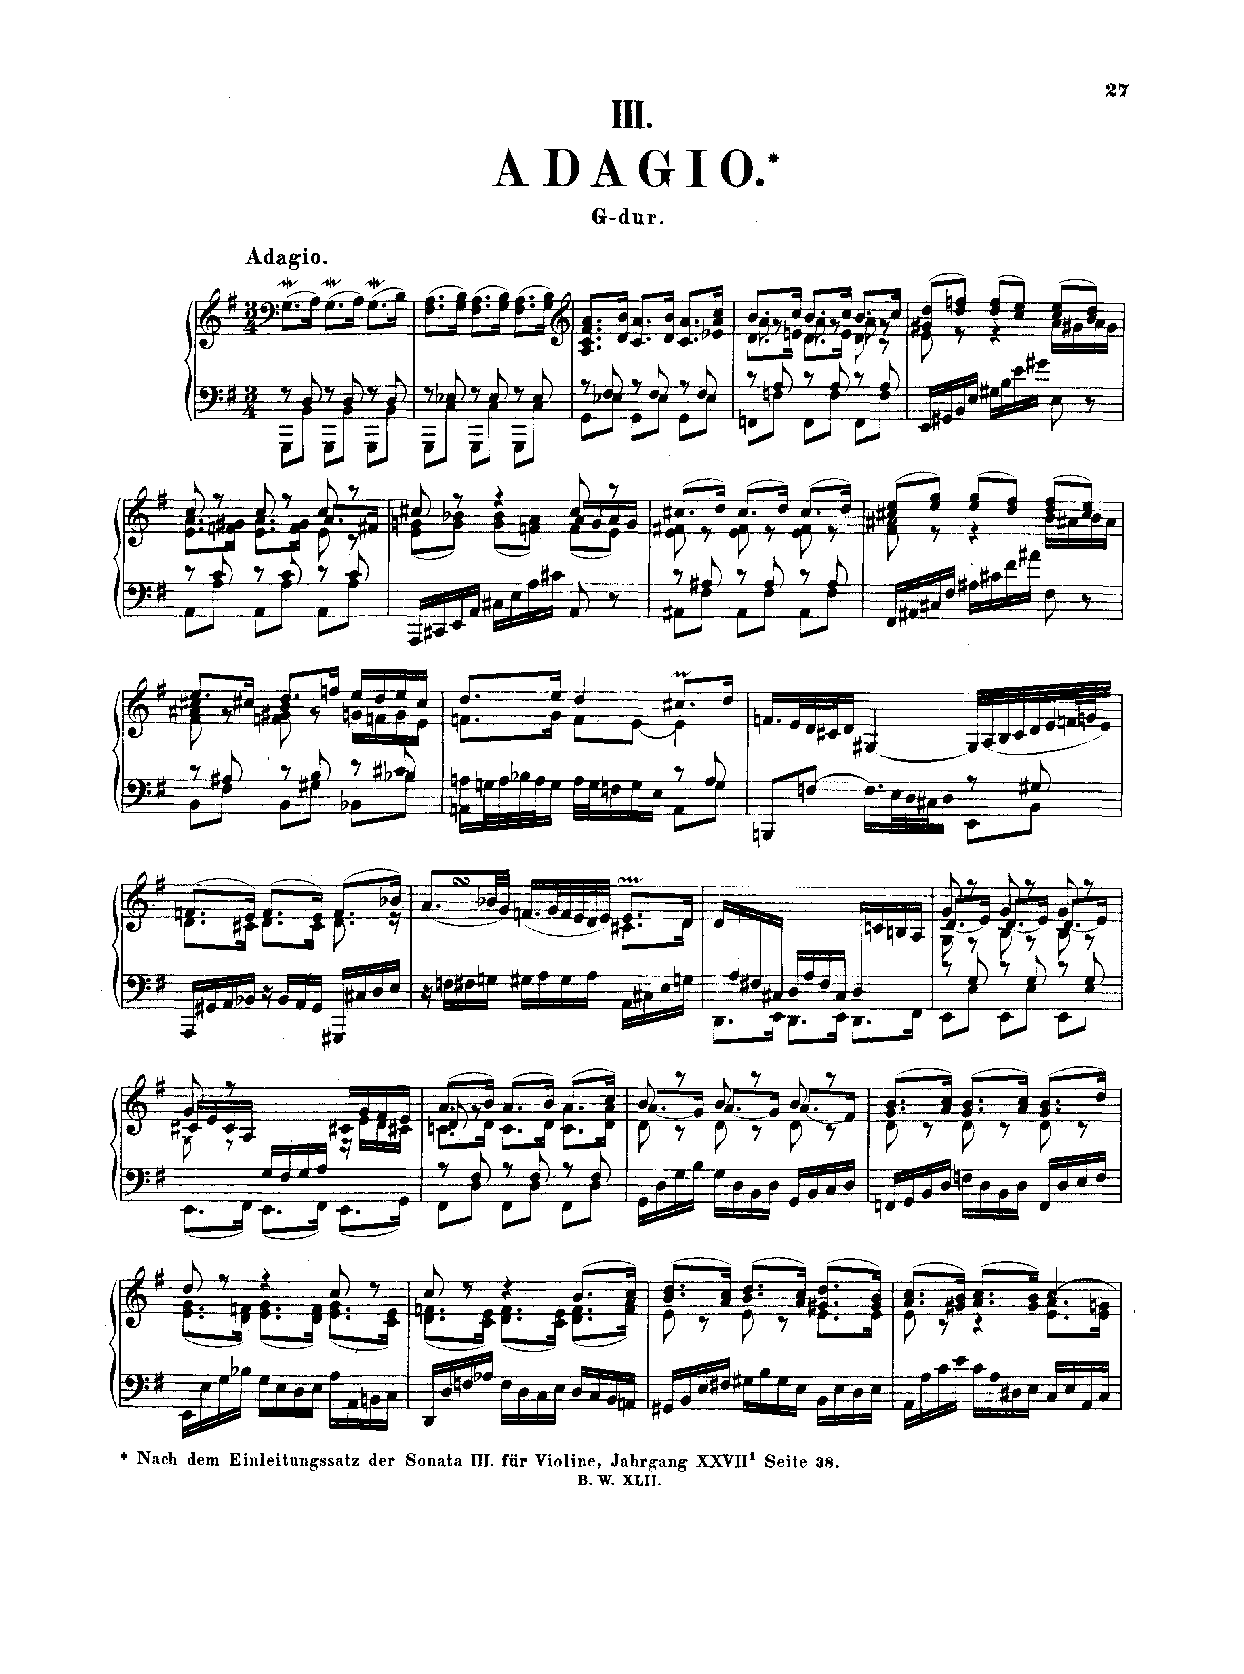
\includegraphics[width=250px,height=125px,keepaspectratio]{bach_adagio}
			\caption{Source: IMLSP Archive}
		\end{figure}


	\end{frame}

	
	\section{Die Techniken}

	\begin{frame}
		\frametitle{Ein graphbasierter Ansatz}
		\begin{minipage}{0.45\textwidth}
			\begin{figure}[h!]
				\fbox{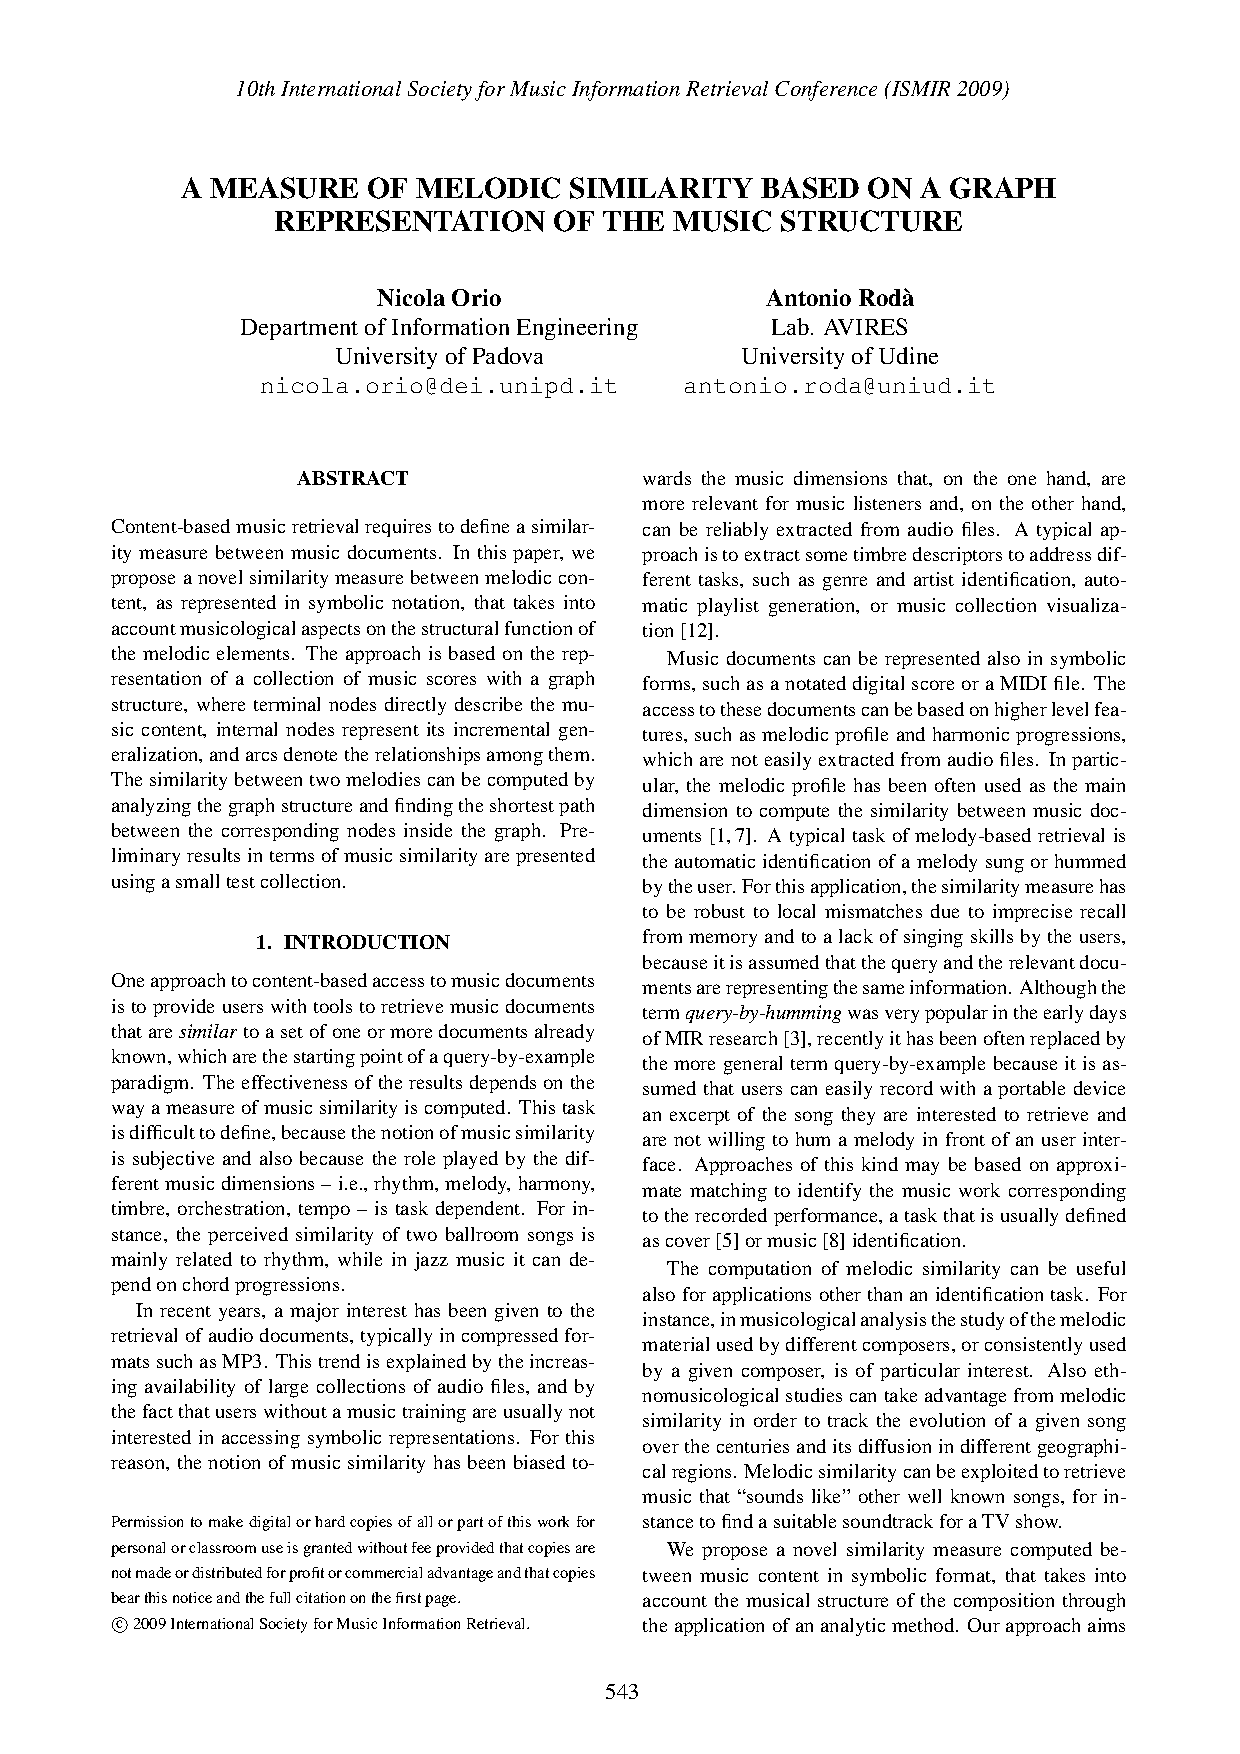
\includegraphics[width=100px,height=100px,keepaspectratio,page=1]{a_measure_of_melodic_similarity_based_on_a_graoh_representation_of_the_music_structure}}
				\footnotemark
			\end{figure}
		\end{minipage}%
		\begin{minipage}{0.45\textwidth}
			\begin{itemize}
				\item Der Inhalt wird schrittweise vereinfacht.
				\note[item]<1>{
							Die Modelle die sich mit der Wahrnehmung von Musik beschäftigt , geht davon aus dass wir Melodien nicht so speichern, wie sie sind sondern vereinfachen wir sie , behalten nur Merkmale.
						}
				\item Dazu sind die \textbf{Gewichte} der einzelnen Noten von Bedeutung.
					\begin{itemize}
						\item die unterliegende harmonische Funktion 
						\item die metrische Position 
						\item die Differenz der Tonlagen zwischen dem Ton und dem Grundton
					\end{itemize}
			\end{itemize}
		\end{minipage}
		\footnotetext[1]{
			\textit{"A Measure of Melodic Similarity Based on a Graph Representation of the Music Structure"} 
			\cite{two_point_four} von Nicola Orio und Antonio Rodá.
		}
	\end{frame}


	\begin{frame}
		\frametitle{Ein graphbasierter Ansatz}
		\begin{figure}[h!]
			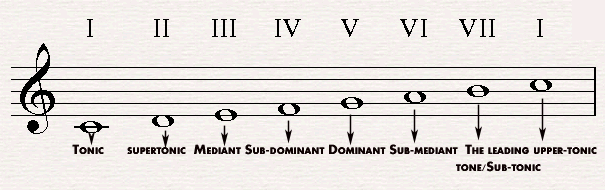
\includegraphics[width=250px,height=125px,keepaspectratio]{functional_degrees}
			\caption{Funktionen der Noten im Tonleiter\cite{functional_degrees_source}} 
			\note[item]<1>{Tonic harmonisch relevanter als Dominant und Dominant als Sub-Dominant usw.}
		\end{figure}
	\end{frame}


	\begin{frame}
		\frametitle{Ein graphbasierter Ansatz}
		\begin{itemize}
				\item Der Inhalt wird schrittweise vereinfacht.
				\note[item]<1>{Jeder Takt wird in jedem Schritt dadurch vereinfacht , dass einige Noten eliminiert sind , und die Bleibenden um die Länge der Eliminierten erweitert werden.}
				\note[item]<1>{Diese Methode heißt Pseudo-Structural Representation (PSR)}
				\item Dazu sind die \textbf{Gewichte} der einzelnen Noten von Bedeutung.
					\begin{itemize}
						\item die unterliegende harmonische Funktion (harmonic weight)
						\item die metrische Position (metric weight)
						\item die Differenz der Tonlagen zwischen dem Ton und dem Grundton(melodic weight)
					\end{itemize}
		\end{itemize}
	\end{frame}

	\begin{frame}
		\frametitle{Ein graphbasierter Ansatz}
		\begin{figure}[h!]
			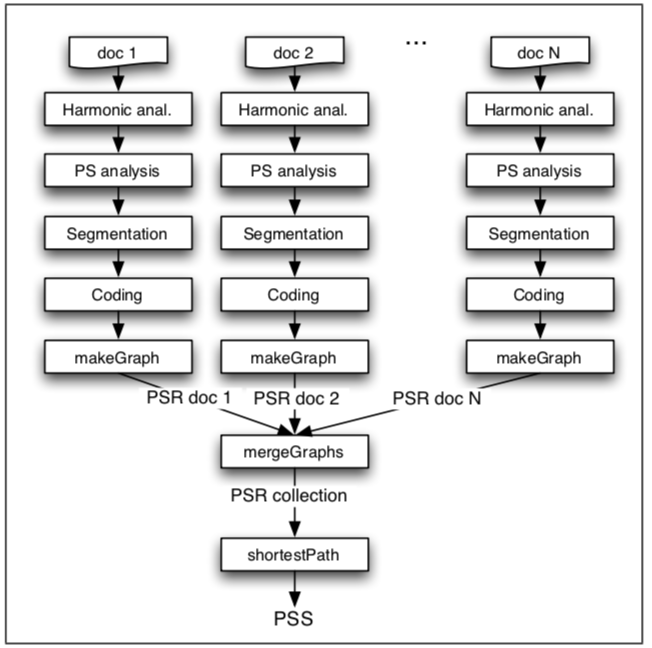
\includegraphics[width=300px,height=150px,keepaspectratio]{four_of_two_point_four}
			\caption{Ablauf des gesamten Verfahren \cite{two_point_four}} 
		\end{figure}
		\note[item]<1>{
			Zuerst wird eine harmonische Analyse durchgeführt. Diese hat die Aufgabe , die Beziehung zwischen Noten zu erkennen.
		}
		\note[item]<1>{
			Die Funktionen der Noten in einem Tonleiter sind nicht immer genau zu bestimmen. Manchmal ist es nicht klar in welchem Kontext zwei Noten zueinander im Verhältnis stehen.
		}
		\note[item]<1>{
			In diesem Paper haben die Autoren deshalb die harmonische Eigenschaften manuell erstellt , was keine positive Eigenschaft ist.
		}
		\note[item]<1>{
			Im zweiten Schritt kommt Vereinfachung hinzu. Der Anfangsmelodie werden die erwähnten Gewichte zugeschrieben.
		}
		\note[item]<1>{
			Nach der Analyse erfolgt die Vereinfachung und dann geht der Algorithmus iterativ weiter , bis nur jeweils eine oder zwei Note in jedem Takt steht.
		}
	\end{frame}

	\begin{frame}
		\frametitle{Ein graphbasierter Ansatz}
			\begin{center}
				\begin{figure}[h!]
					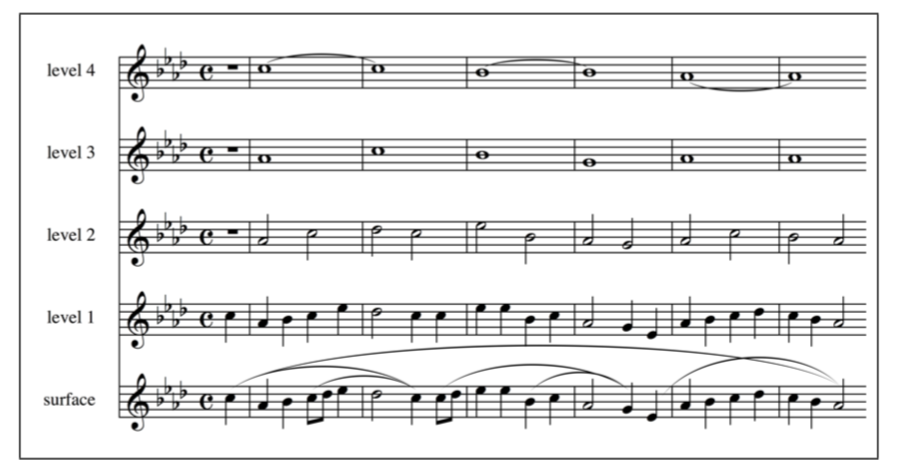
\includegraphics[width=300px,height=100px,keepaspectratio]{one_of_two_point_four}
				\end{figure}
			\end{center}

			\begin{center}
				\begin{figure}[h!]
				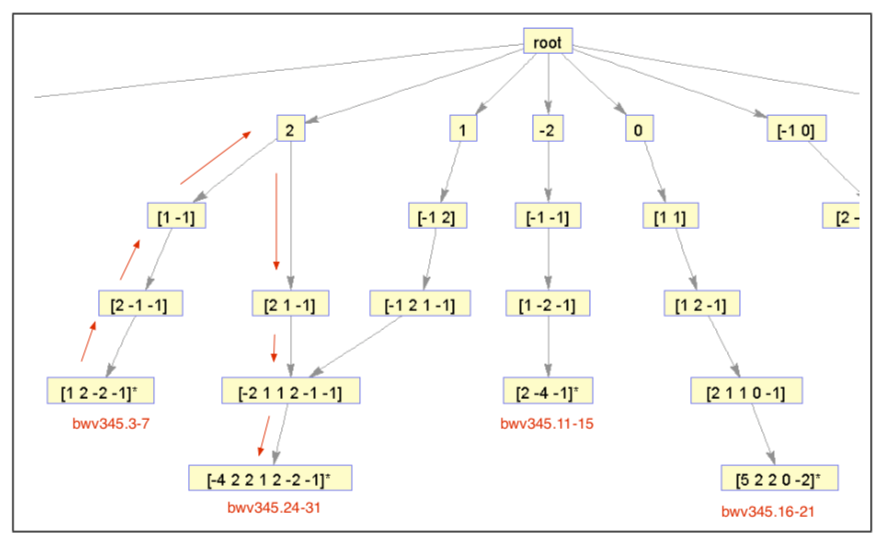
\includegraphics[width=300px,height=100px,keepaspectratio]{two_of_two_point_four}
				\end{figure}
			\end{center}

			\note[item]<1>{
				Dies stellt eine Metrik dar: Es ist positiv-definiert , symmetrisch und die Dreieicksungleichung gilt offenbar.
			}
	\end{frame}

	\begin{frame}
		\frametitle{Ein graphbasierter Ansatz}
		\begin{figure}[h!]
					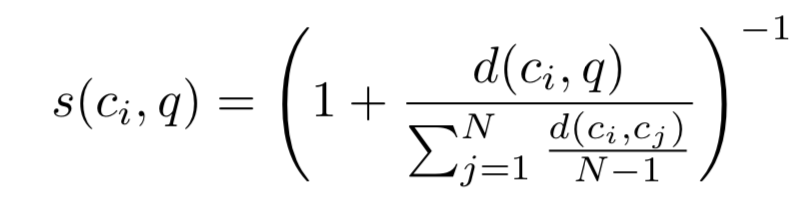
\includegraphics[width=300px,height=100px,keepaspectratio]{five_of_two_point_four}
		\end{figure}
		\note[item]<1>{
			$d(c_i,c_j)$ : Wir gucken , was die Distanzen zwischen Segmenten von den beiden Dokumenten sind.
		}
		\note[item]<1>{
			Nehmen dann den Median und der Medianwert bildet dann die Distanz. Dieser Wert wird dann normalisiert , indem er durch die durchschnittliche Distanz des Dokuments $c_i$
			zu allen anderen Dokumenten in der Sammlung geteilt wird. Die Werte zur Normalisierung können im Voraus berechnet werden.
		}
	\end{frame}

	\begin{frame}
		\frametitle{Evaluierung}
		\begin{itemize}
			\item RISM-Sammlung
			\item Basiswissen von Experten als Maßstab
		\end{itemize}
	\end{frame}

	\begin{frame}
		\frametitle{LBDM}
		\begin{itemize}
			\item Local Boundary Detection Model
			\item Change Rule (CR) : Je größer die Differenz , desto wahrscheinlicher wird die Nichtzusammengehörigkeit.
			\item Proximity Rule (PR) : Change Rule angewandt auf Intervalle.
		\end{itemize}
	\end{frame}

	\begin{frame}
		\frametitle{Ähnliche Anwendung der Gestaltstheorie}
		\begin{minipage}{0.45\textwidth}
			\begin{figure}[h!]
				\fbox{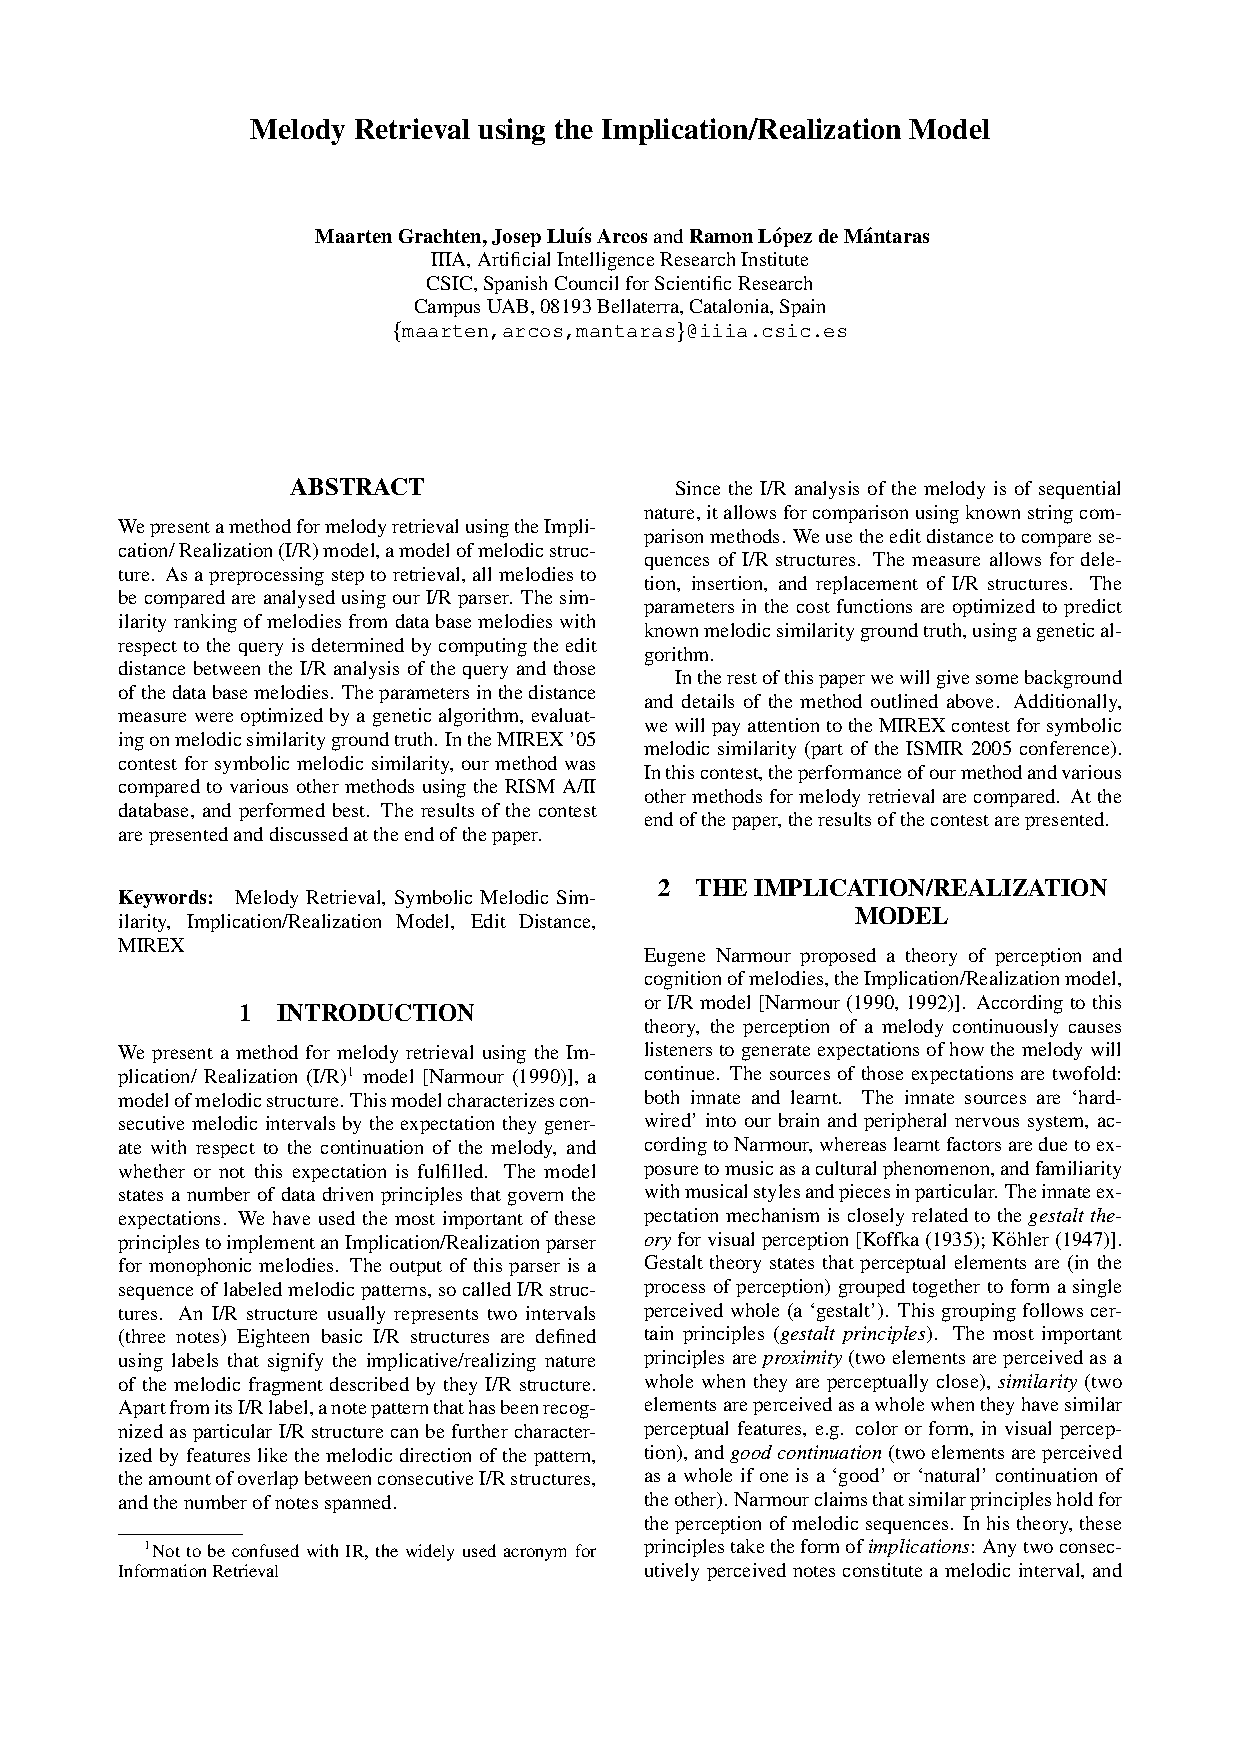
\includegraphics[width=100px,height=100px,keepaspectratio,page=1]{mirex_2005_one.pdf}}
				\footnotemark
			\end{figure}
		\end{minipage}%
		\begin{minipage}{0.45\textwidth}
			\begin{itemize}
				\item Implication/Realization Model.
				\item Dies besagt , dass man nach seinen Erfahrungen (sowohl kulturellen , als auch angeborenen) Erwartungen hat , wie ein Musikstück weitergeht. 
				\item Wir beschäftigen uns hier mit den angeborenen Aspekten.
			\end{itemize}
		\end{minipage}
		\footnotetext[1]{
			\textit{"Melody Retrieval using the Implication/Realization Model"} 
			\cite{mirex_2005_one} Maarten Grachten, Josep Lluis Arcos and Ramon Lopez de Mantaras 
		}
	\end{frame}
	\begin{frame}
		\frametitle{Ähnliche Anwendungen der Gestaltstheorie}
		\begin{itemize}
			\item I/R Modell besagt : Wir sind dazu geneigt , Elemente nach Konzepten zu gruppieren. Diese Konzepten sind denen der Gestalttheorie ähnlich
					\begin{itemize}
						\item Proximity : Werden zwei Elemente gleich wahrgenommen?
						\item Similarity : Haben zwei Elemente Ähnlichkeiten?
					\end{itemize}
			\item PRD : kleines Intervall in eine Richtung impliziert noch ein Intervall in dieselbe Richtung
			\item PID : kleines Intervall impliziert ein kleines Intervall.
			\item Nach diesen Prinzipien ist ein Alphabet von Strukturen definiert.
			\item Mithilfe von Edit Distance wird die Ähnlichkeit festgestellt.
		\end{itemize}
	\end{frame}

	\begin{frame}
		\frame{Diskussion}

		\begin{itemize}
			\item hey
		\end{itemize}
	\end{frame}
	
    \begin{frame}
		\frametitle{Ein mathematischer Ansatz}
		\begin{minipage}{0.45\textwidth}
			\begin{center}
				\textit{"Algorithms for Computing Geometric Measures of Melodic Similarity"} 
				\cite{one}  \\ 
				von Greg Aloupis, Thomas Fevens, Stefan Langerman, Tomomi Matsui, Antonio Mesa, Yurai Nunez, David Rappaport, and Godfried Toussaint
			\end{center}
		\end{minipage}%
		\begin{minipage}{0.45\textwidth}
			\begin{figure}[h!]
				\fbox{\includegraphics[width=100px,height=100px,keepaspectratio,page=2]{algorithms_for_computing_geometric_measures_of_melodic_similarity}}
			\end{figure}
		\end{minipage}
	\end{frame}
	
	\begin{frame}
        \frametitle{Ein mathematischer Ansatz}
        \begin{minipage}{0.45\textwidth}
            \begin{itemize}
             \item Melodien werden als Polygonalketten dargestellt
             \item Tonlänge wird durch Länge der waagerechten Kanten modelliert
             \item Intervalle werden durch Länge der senkrechten Kanten modelliert 
            \end{itemize}
        \end{minipage}
        \begin{minipage}{0.45\textwidth}
        \begin{figure}[h!]
            \fbox{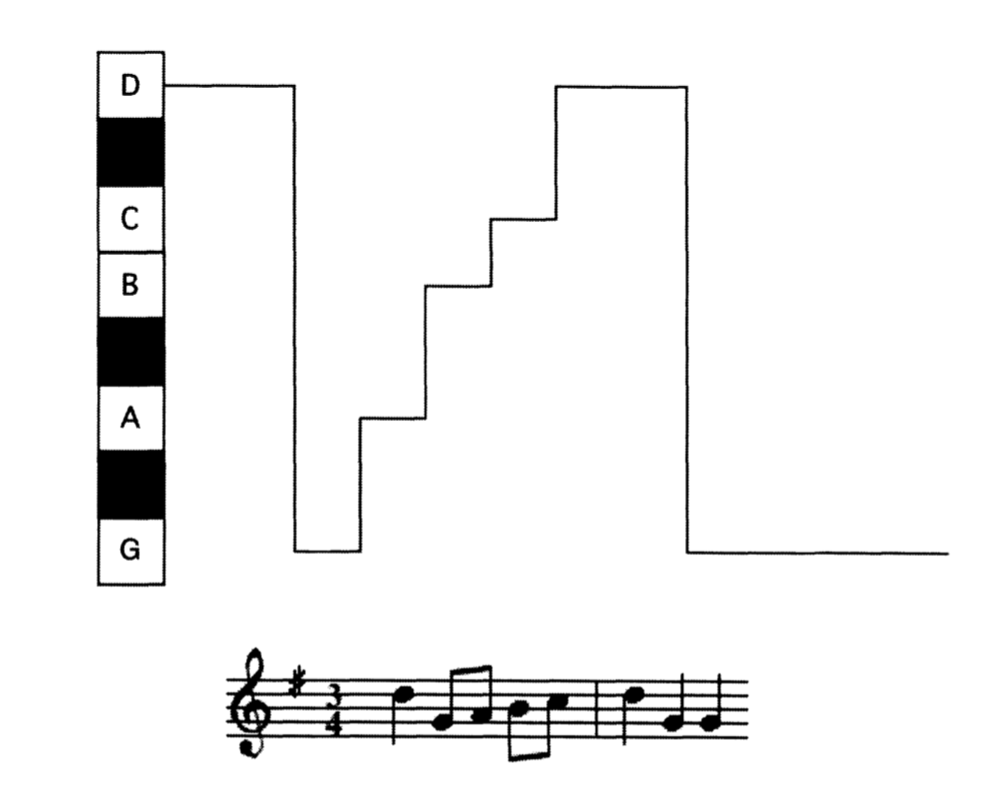
\includegraphics[width=150px,height=150px,keepaspectratio]{abb_1}}
             \caption{Source: \cite{one}}
        \end{figure}
        \end{minipage}
	\end{frame}

	\begin{frame}
        \frametitle{Ein mathematischer Ansatz}
        \begin{figure}[h]
       	\fbox{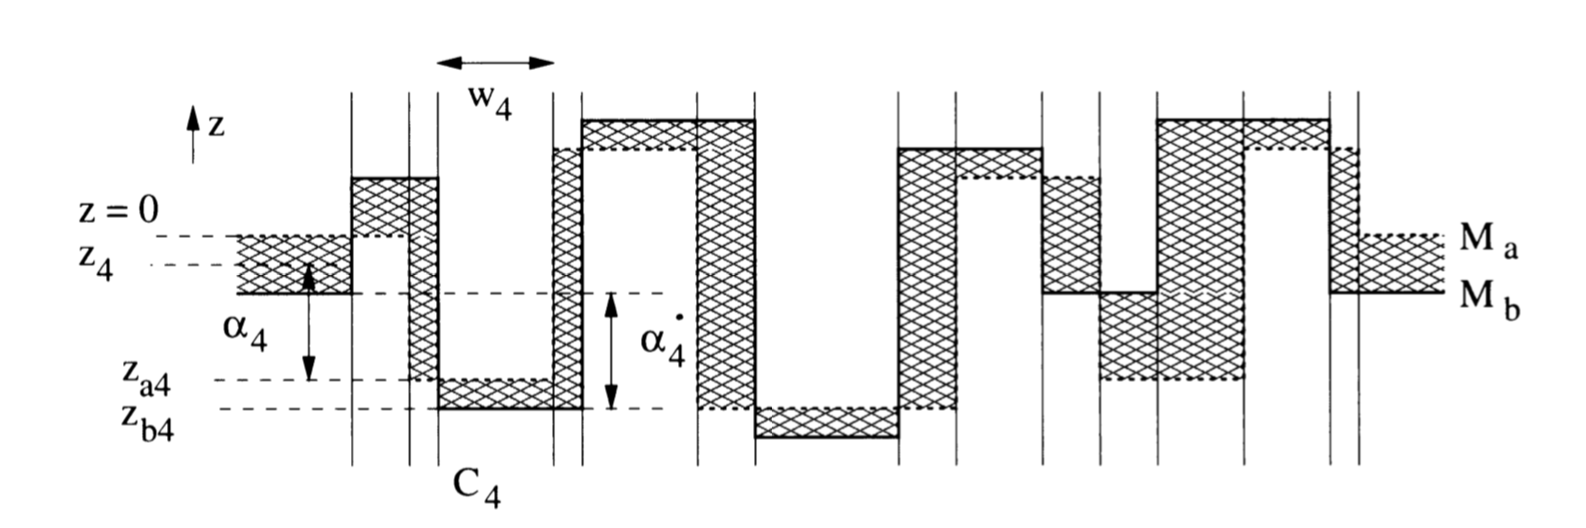
\includegraphics[width=0.7\textwidth]{abb_2}}%
        \fbox{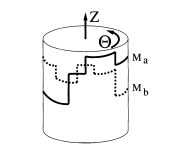
\includegraphics[width=0.3\textwidth]{abb_3}}
        \caption{Source: \cite{one}}
        \end{figure}
	\end{frame}

	\section{MIREX : Algorithmen treten gegeneinander an}

	\begin{frame}
		\frametitle{MIREX}
		\begin{itemize}
			\item Ein Wettbewerb und Plattform für Interessierte
			\item Verschiedene Kategorien
				\begin{itemize}
					\item Real-time Audio to Score Alignment (a.k.a Score Following)
					\item Discovery of Repeated Themes and Sections
					\item Audio Melody Extraction
					\item \textbf{Symbolic Melodic Similarity}
					\item ...
				\end{itemize}
			\item Welche Messmethoden gibt es , um den Erfolgt eines Algorithmus festzustellen?
		\end{itemize}
	\end{frame}

	\begin{frame}
		\frametitle{MIREX}
		\begin{figure}[h!]
			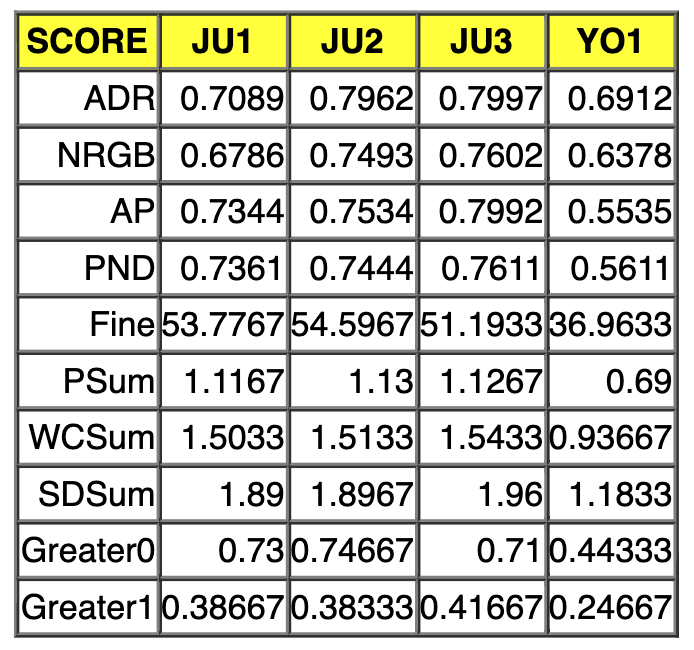
\includegraphics[width=300px,height=150px,keepaspectratio]{MIREX_2014_results}
			\caption{Source: \cite{mirex_website_2014_results}}
		\end{figure}
	\end{frame}


	\subsection{Ground Truth}
		
		\begin{frame}
			\frametitle{Ground Truth}
			\begin{itemize}
				\item Experten werden befragt , Stücke aus der RISM A/II Sammlung  nach deren Ähnlichkeiten zu einer Anfrage zu beurteilen.
				\item Die Sammlungen sind groß deswegen sind einige Techniken zur Eliminierung unrelevanter Elementen vorzunehmen , wie z.B
					\begin{itemize}
						\item Nach der Differenz zwischen dem tiefsten und höchsten Ton.
						\item Nach dem Verhältnis der kürzesten Note zu der längsten.
						\item usw.
					\end{itemize}
				\item Nicht für alle Stücke werden dieselben Elimierungsverfahren vorgenommen. Die Aspekte , durch die sich ein Stück auszeichnet sind beizubehalten. Das ist wiederum für die Experten zu entscheiden.
			\end{itemize}
		\end{frame}

		\begin{frame}[allowframebreaks]
			\frametitle{Ground Truth}
				\begin{figure}[h!]
					
\includegraphics[width=300px,height=75px,keepaspectratio]{ground_truth_query}
					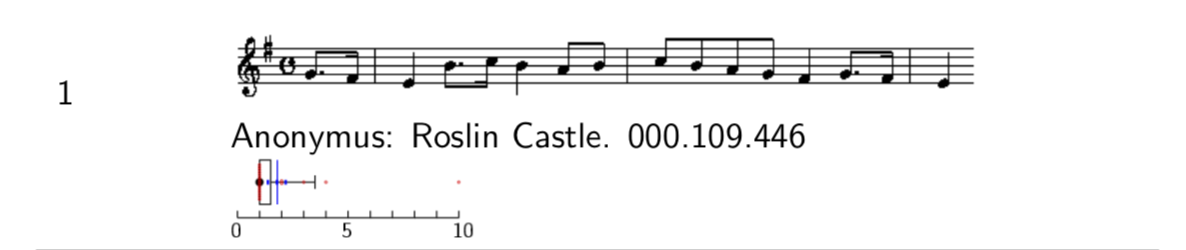
\includegraphics[width=300px,height=75px,keepaspectratio]{ground_truth_results_one}
					\caption{Abbildung: Ergebnisse der Befragung \cite{three}}
				\end{figure}
				\begin{figure}[h!]
					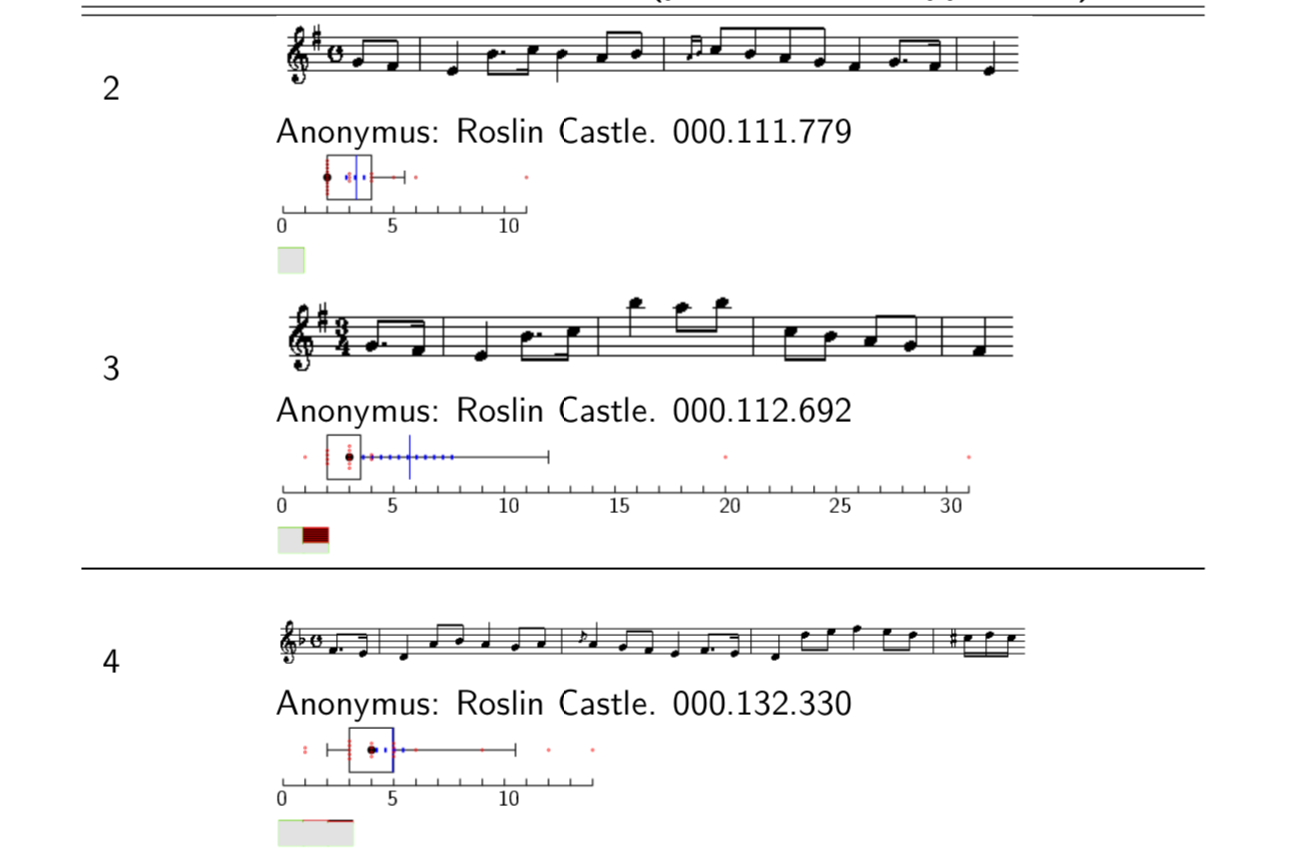
\includegraphics[width=300px,height=150px,keepaspectratio]{ground_truth_results_two}
				\end{figure}
				\begin{figure}[h!]
					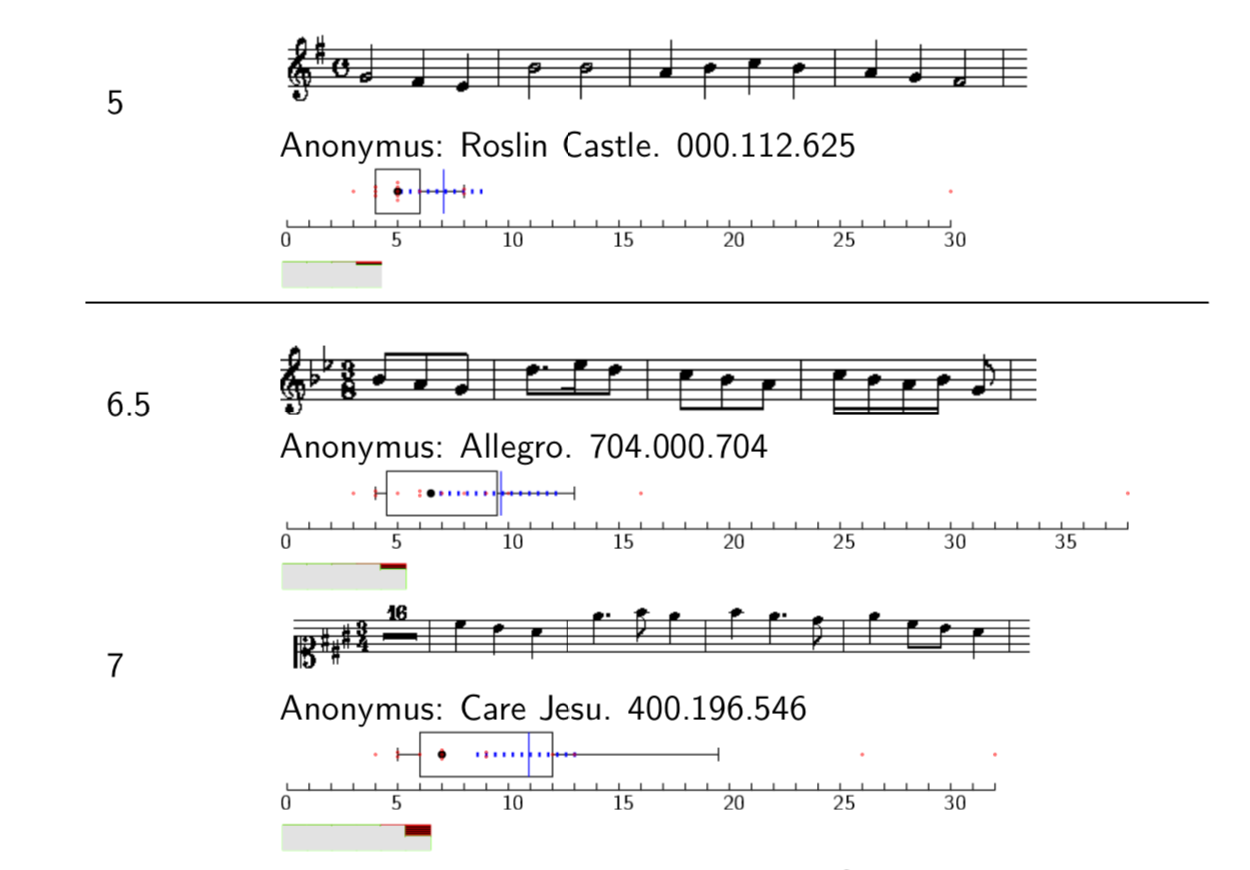
\includegraphics[width=300px,height=150px,keepaspectratio]{ground_truth_results_three}
				\end{figure}
		\end{frame}

	\begin{frame}
		\frametitle{MIREX}
		\begin{figure}[h!]
			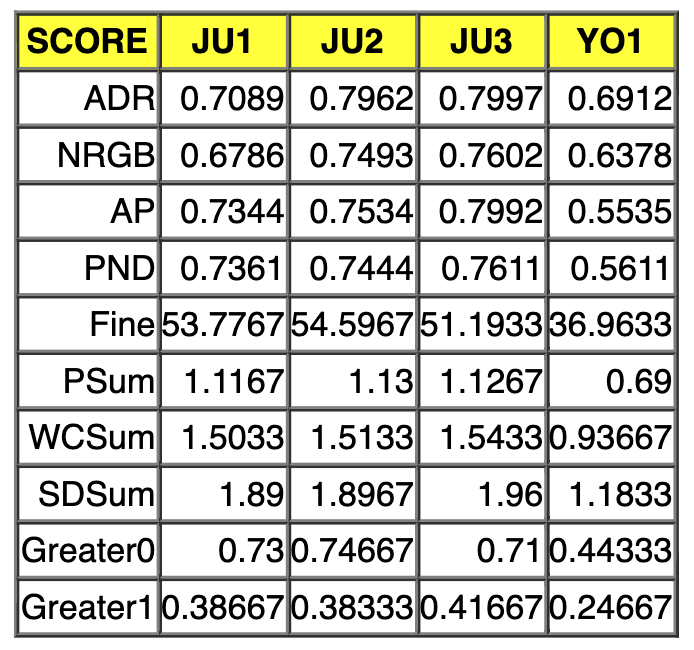
\includegraphics[width=300px,height=150px,keepaspectratio]{MIREX_2014_results}
			\caption{Source: \cite{mirex_website_2014_results}}
		\end{figure}
	\end{frame}


	\subsection{Average Dynamic Recall}

		\begin{frame}
			\frametitle{Beispiel : Average Dynamic Recall - ADR}

			Betrachte die Gruppierungen $\langle(1,2),(3,4,5)\rangle$ und die Ergebnisse $(2,3,1,5,7,8,9,4)$

			\begin{figure}[h!]
				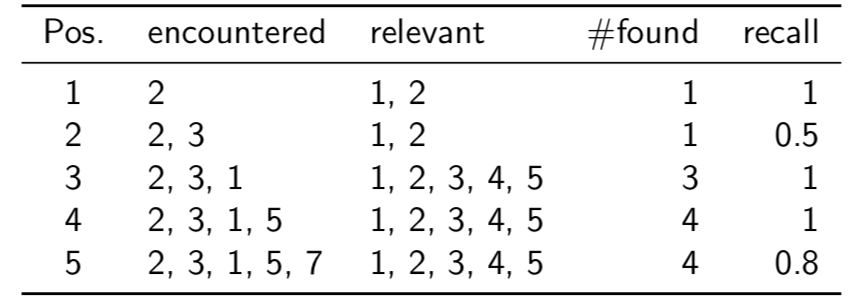
\includegraphics[width=300px,height=150px,keepaspectratio]{adr_example}
				\caption{Abbildung: ADR Berechnung \cite{three}}
			\end{figure}
		\end{frame}


	\subsection{MIREX 2014}
	\begin{frame}
		\frametitle{Ähnlichkeitssuche durch Pattern Mining}
		\begin{minipage}{0.45\textwidth}
			\begin{figure}[h!]
				\fbox{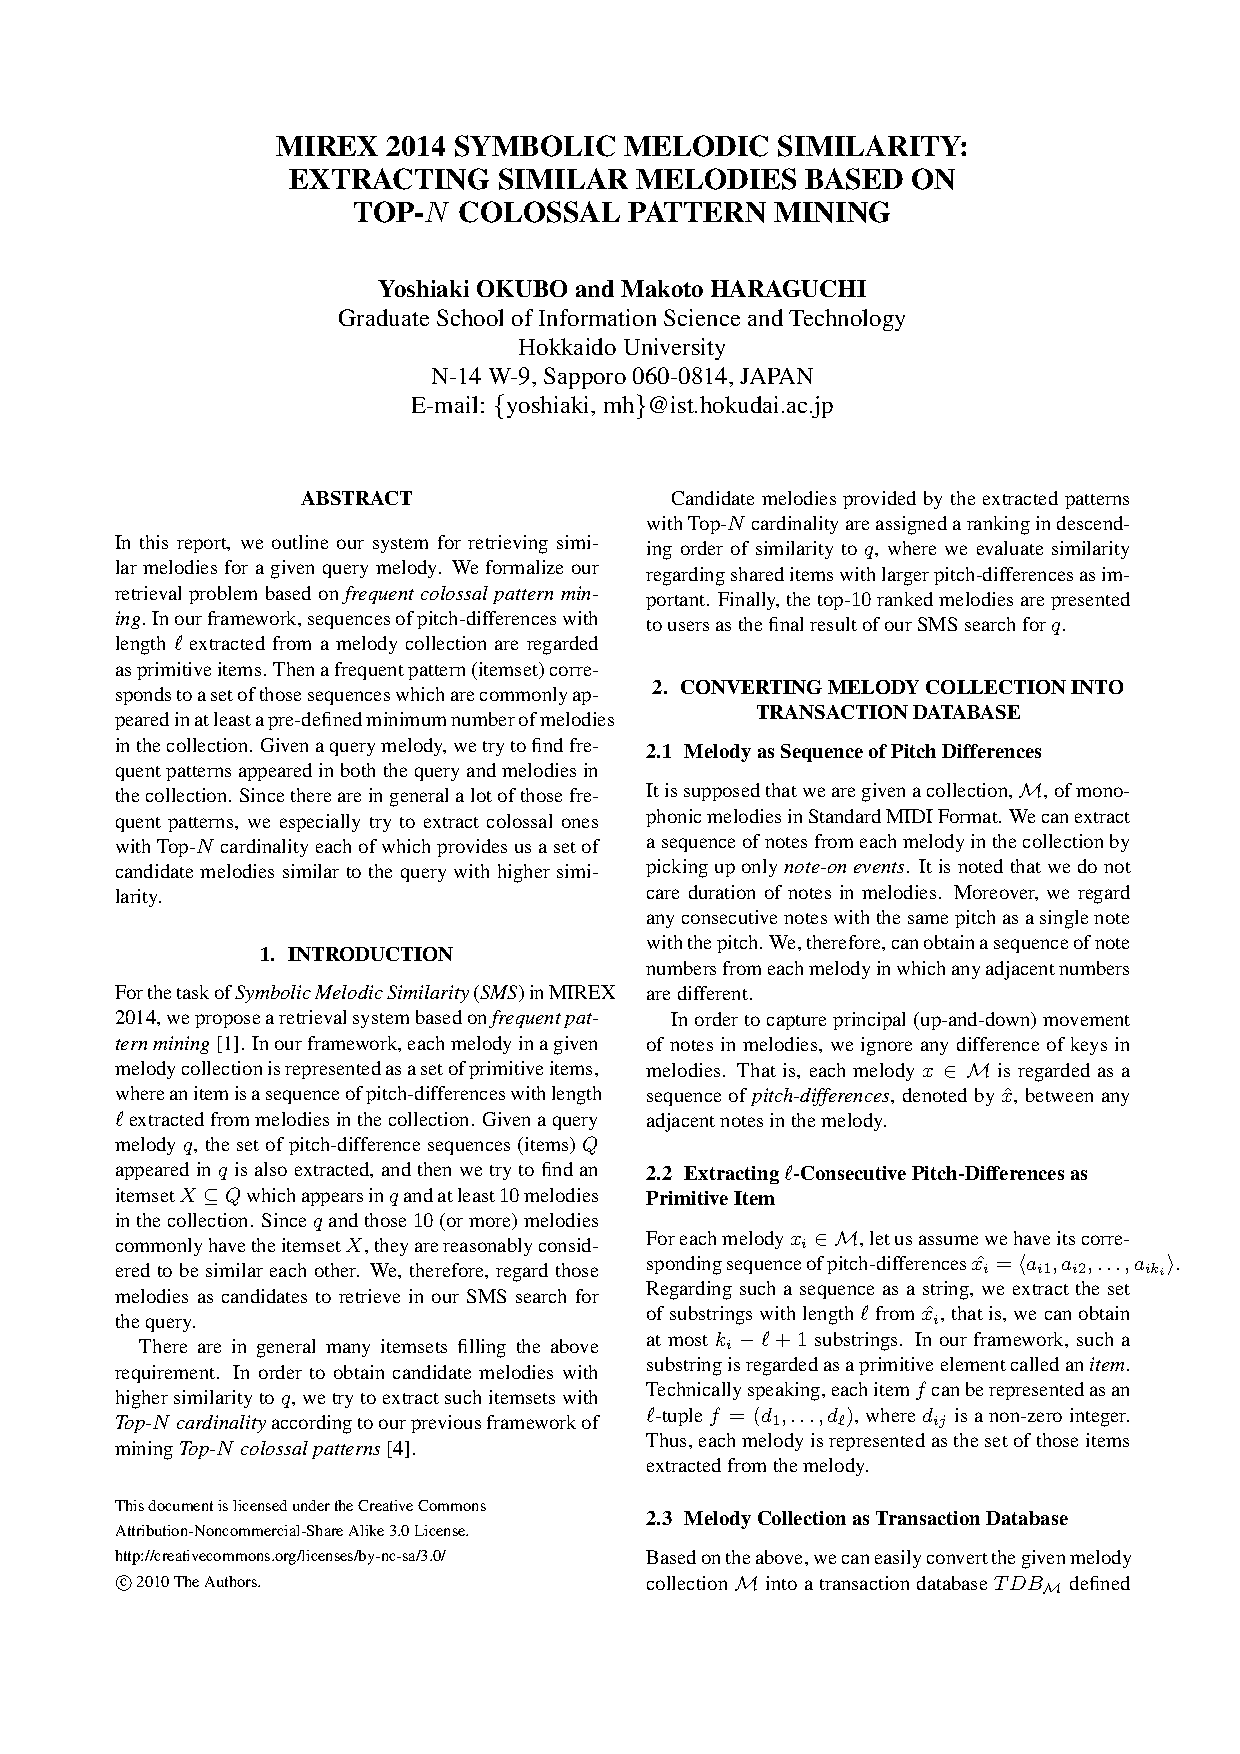
\includegraphics[width=100px,height=100px,keepaspectratio,page=1]{YO1}}
				\footnotemark
			\end{figure}
		\end{minipage}%
		\begin{minipage}{0.45\textwidth}
			\begin{itemize}
				\item Nur Note-On Events
				\item Dauer einer Note spielt keine Rolle.
				\note[item]<1>{
					Obwohl es nachgewiesen ist , dass die Tonlage wichtigsten Aspekt der Wahrnehmung der Musik bildet , ist es immer noch keine gute Idee die restlichen Aspekte komplett zu vernachlässigen.
				}
				\item Grundton spielt keine Rolle. Es werden die Differenzen zwischen Tonlagen in Betracht gezogen. 
				\item Jede Melodie wird durch primitive 'Items' dargestellt.
			\end{itemize}
		\end{minipage}
		\footnotetext[1]{
			\textit{"MIREX 2014 Symbolic Melodic Similarity : Extracting Similar Melodies Based on Top-N Colossal Pattern Mining"}
			\cite{MIREX_2014_one} von Shiho Sugimoto, Yuto  Nakashima, Masayuki Takeda.
		}
	\end{frame}


	\begin{frame}
		\frametitle{Ähnlichkeitssuche durch Pattern Mining}

		\begin{itemize}
			\item Einer Melodie werden alle N-Gramme entnommen.
			\item $TDB_M =  \{ (ID(x) , trans(x)) | x \in M \}$
		\end{itemize}
	\end{frame}

	\begin{frame}
		\frametitle{Diskussion}
		\begin{itemize}
			\item Kann man rhytmische Werte vernachlässigen ?
			\item Was ist das richtige n für das N-Gramm?
		\end{itemize}
	\end{frame}
	
	
	\subsection{Urbano MelodyShape}
		\begin{frame}
			\frametitle{Urbano MelodyShap}
			\begin{minipage}{0.45\textwidth}
				\begin{center}
					\textit{"MelodyShape at MIREX 2014 Symbolic Melodic Similarity"} 
					\cite{five_point_two}\\ 
					von Julian Urbano
				\end{center}
			\end{minipage}%
			\begin{minipage}{0.45\textwidth}
				\begin{figure}[h!]
					\fbox{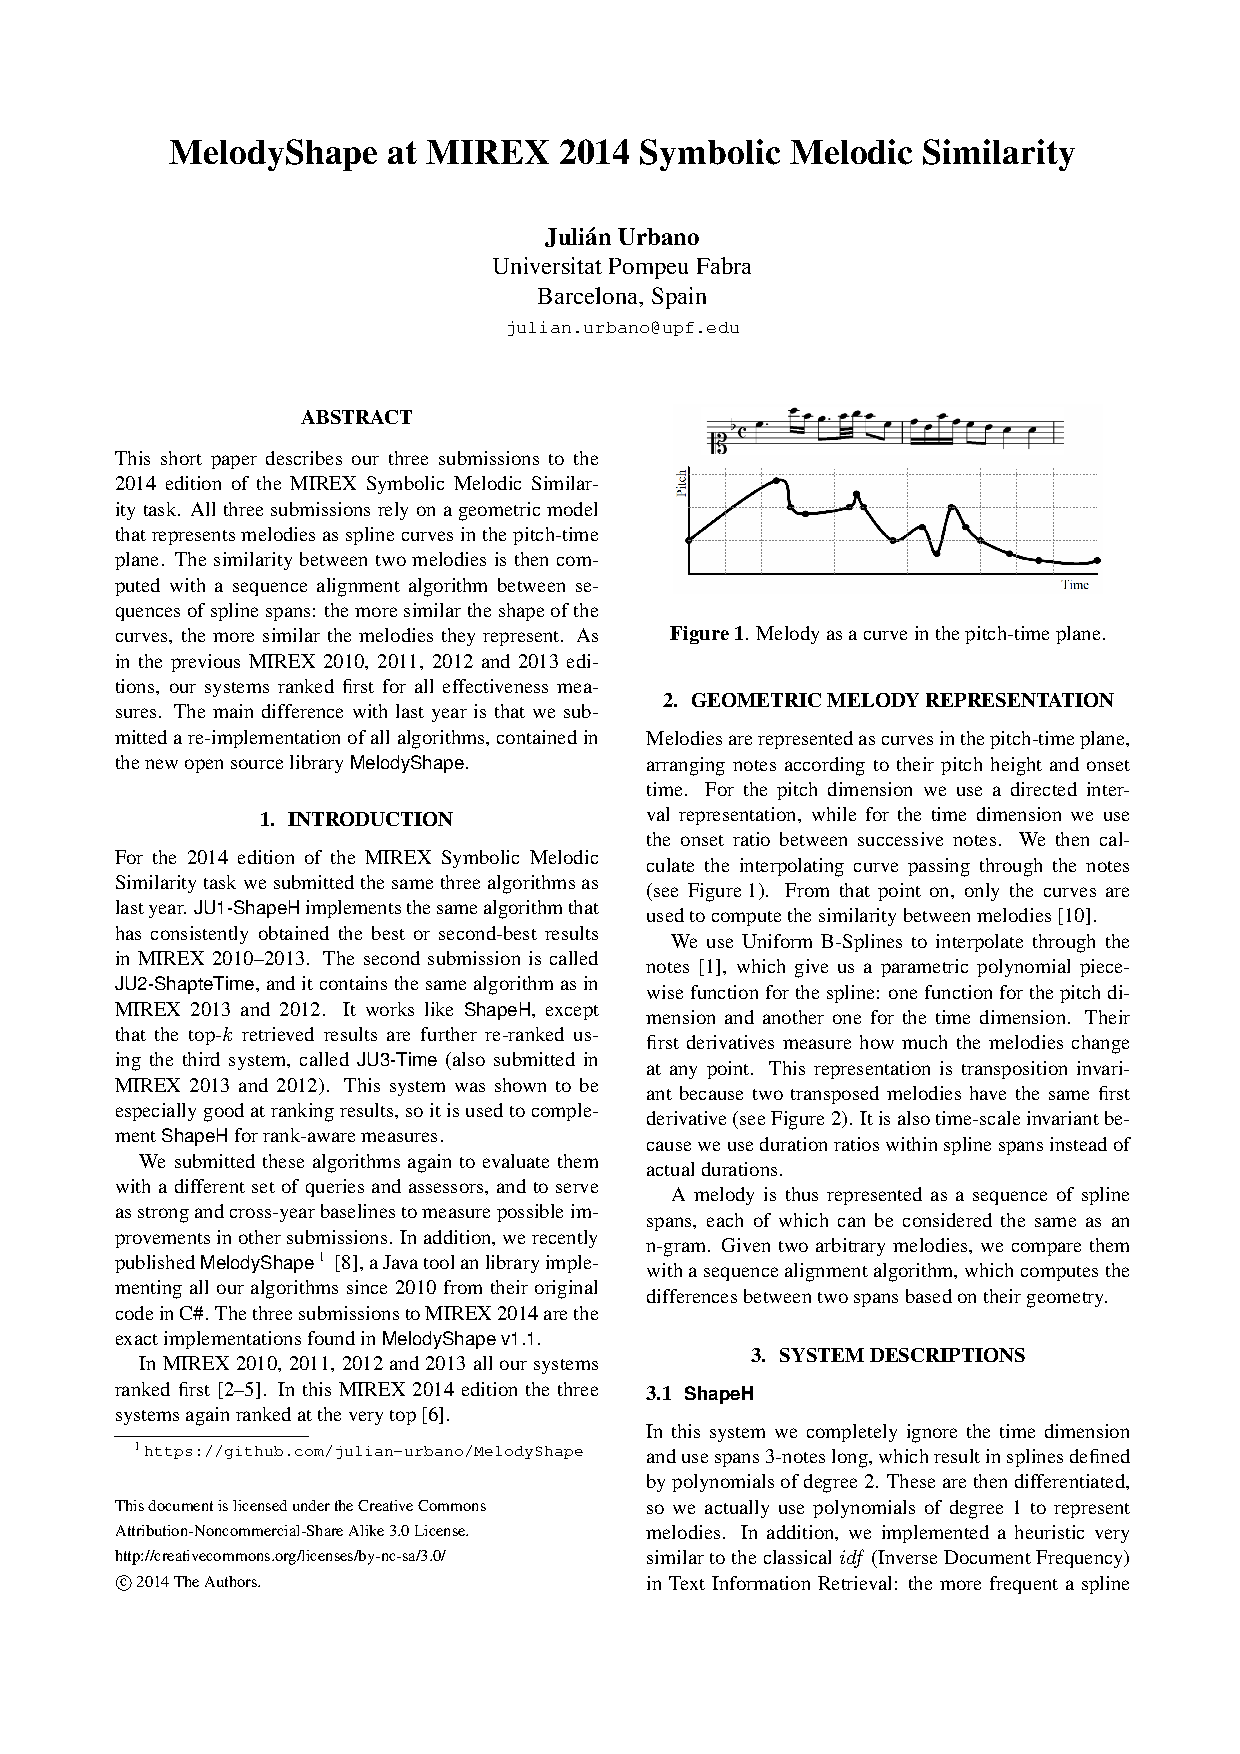
\includegraphics[width=100px,height=100px,keepaspectratio,page=1]{JU1}}
				\end{figure}
			\end{minipage}
		\end{frame}
		
	\begin{frame}
        \frametitle{Urbano MelodyShape}
        \begin{minipage}{0.45\textwidth}
            \begin{itemize}
             \item Töne werden als Punkt  auf Pitch-Time plane dargestellt.
             \item Darstellung als Funktion durch Interpolation mithile von Splines.
            \end{itemize}
        \end{minipage}
        \begin{minipage}{0.45\textwidth}
        \begin{figure}[h!]
            \fbox{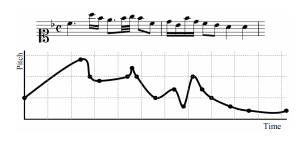
\includegraphics[width=150px,height=150px,keepaspectratio]{abb_4}}
             \caption{Source: \cite{five_point_two}}
        \end{figure}
        \end{minipage}
	\end{frame}
	
    \begin{frame}
        \frametitle{Needlemann - Wunsch Algorithmus}
      \begin{figure}[h!]
       \fbox{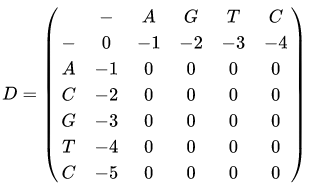
\includegraphics[width=0.5\textwidth]{abb_7}}%
        \fbox{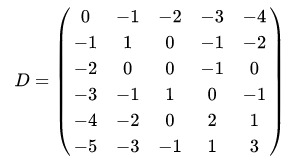
\includegraphics[width=0.5\textwidth]{abb_8}}
         \caption{Source: \cite{wiki_nee_wu}}
        \end{figure}
	\end{frame}
	
	\begin{frame}
        \frametitle{ShapeH}
        \begin{minipage}{0.45\textwidth}
            \begin{itemize}
             \item Insertion : $ s(-, n) = -(1 - f(n))$
             \item Deletion: $s(n, -) = -(1 - f(n))$
             \item Match: $s(n, n) = 1 - f(n)$
     %        \item Sequence Alignment $H(i,j) = max \{H(i - 1, j - 1) + s(a_i,b_j) \n
        %     H(i - 1, j) + s(a_i, -) \n H(i, j - 1) + s(i, b_j) \}$
            \end{itemize}
        \end{minipage}
        \begin{minipage}{0.45\textwidth}
        \begin{figure}[h!]
            \fbox{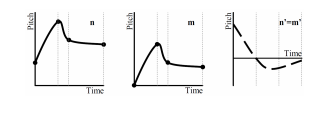
\includegraphics[width=150px,height=150px,keepaspectratio]{abb_5}}
             \caption{Source: \cite{five_point_two}}
        \end{figure}
        \end{minipage}
	\end{frame}
	
	\begin{frame}
        \frametitle{Time}
            \begin{itemize}
             \item Insertion : $ s(-, n) = -diff_p(n,\Theta (n)) - \lambda k_t * diff_t(n,\Theta (n))$
             \item Deletion: $s(n, -) = -diff_p(n,\Theta (n)) - \lambda k_t * diff_t(n,\Theta (n))$
             \item Match: $2\mu_p + 2\lambda k_t\mu_t = 2\mu_p(1+k_t)$
             \item Substitution $s(n,m) = -diff_p(n,m) - \lambda k_t * diff_t(n,m)$
            \end{itemize}
            \begin{center}
            \begin{figure}[h!]
            \fbox{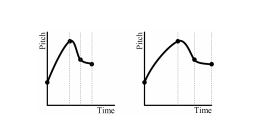
\includegraphics[width=150px,height=150px,keepaspectratio]{abb_6}}
             \caption{Source: \cite{five_point_two}}
            \end{figure}
            \end{center}
	\end{frame}
	


	\section{Bibliographie}
	\begin{frame}[allowframebreaks]
		\frametitle{Bibliographie}
		\begin{thebibliography}{5}
			\setbeamertemplate{bibliography item}[text]
			\bibitem[1]{duden_melodie} Duden: Melodie: Rechtschreibung, Bedeutung, Definition, Herkunft
			https://www.duden.de/rechtschreibung/Melodie.
			\bibitem[2]{duden_harmonie} Duden: Harmonie : Rechtschreibung, Bedeutung, Definition, Herkunft
			https://www.duden.de/rechtschreibung/Harmonie.
			\bibitem[3]{def_schlussel} “Notenschlüssel.” Wikipedia, Wikimedia Foundation, 11 Dec. 2019, de.wikipedia.org/wiki/Notenschlüssel.
			\bibitem[4]{mirex_website} MIREX,Symbolic Melodic Similarity 2005,https://www.music-ir.org/mirex/wiki/2005:Symbolic\_Melodic.
			\bibitem[5]{mirex_website_2014_results} MIREX,Symbolic Melodic Similarity Results 2014, https://www.music-ir.org/mirex/wiki/2014:Symbolic\_Melodic\_Similarity\_Results.
			\bibitem[6]{three} Typke, Rainer. (2007). Music Retrieval based on Melodic Similarity.
			\bibitem[7]{two_point_four} Orio, N., and A. Rodá. 2009. “A Measure of Melodic Similarity Based on a Graph Representation of the Music Structure.” In Proceedings of the International Conference for Music Information Retrieval, pp. 543– 548.
			\bibitem[8]{one} Greg Aloupis, Thomas Fevens, Stefan Langerman, Tomomi Matsui, Antonio Mesa, Yurai Nunez, David Rappaport, and Godfried Toussaint, "Algorithms for Computing Geometric Measures of Melodic Similarity" Computer Music Journal, Vol.30, No. 3 (Autumn, 2006), pp. 67-76
			\bibitem[9]{functional_degrees_source} Tonal Degrees [Online]. [Accessed 30 Jan 2020]. Available from : http://www.piano-play-it.com/musical-scales.html
			\bibitem[10]{five_point_two} J. Urbano. MelodyShape at MIREX 2014 Symbolic
            Melodic Similarity. Technical report, Music Information Retrieval Evaluation eXchange, 2014
           	\bibitem[13]{wiki_nee_wu} Wikipedia, Needlemann-Wunsch-Algorithmus, https://de.wikipedia.org/wiki/Needleman-Wunsch-Algorithmus, abgerufen am 02.02.20
           	\bibitem[14]{MIREX_2014_one} Okubo Yoshiaki , Haraguchi Makoyo , "MIREX 2014 Symbolic Melodic Similarity : Extracting Similar Melodies Based on Top-N Colossal Pattern Mining". Technical report, Music Information Retrieval Evaluation eXchange, 2014
		\end{thebibliography}
	\end{frame}
\end{document}
